\documentclass[a4paper,12pt]{article}

\usepackage{fontspec}
\usepackage{polyglossia}
\setmainfont{Times New Roman}
\setsansfont{Arial}
\setmonofont{Courier New}
\setdefaultlanguage{russian}
\newfontfamily\cyrillicfont{Times New Roman}
\newfontfamily\cyrillicfontsf{Arial}
\newfontfamily\cyrillicfonttt{Courier New}
\usepackage{geometry}
\usepackage{amsmath,amssymb}
\usepackage{graphicx}
\usepackage{float}
\usepackage{caption}
\usepackage{booktabs}
\usepackage{array}
\usepackage{xcolor}
\usepackage{listings}
\usepackage{hyperref}
\usepackage{tikz}
\usetikzlibrary{arrows.meta,positioning,shapes.geometric}

\geometry{left=2cm,right=2cm,top=2cm,bottom=2cm}
\captionsetup[figure]{name=Рисунок}
\captionsetup[table]{name=Таблица}
\hypersetup{colorlinks=true,linkcolor=black,urlcolor=blue}
\setlength{\parindent}{1.25cm}
\setlength{\parskip}{0.15cm}
\setlength{\emergencystretch}{2em}

\lstset{
    basicstyle=\ttfamily\small,
    keywordstyle=\color{blue!70!black}\bfseries,
    commentstyle=\color{gray}\itshape,
    stringstyle=\color{red!70!black},
    numbers=left,
    numberstyle=\tiny\color{gray},
    numbersep=8pt,
    frame=single,
    breaklines=true,
    showstringspaces=false,
    tabsize=4
}

\begin{document}

\begin{titlepage}
    \centering

    {\small
        Министерство науки и высшего образования Российской Федерации\\
        Федеральное государственное автономное образовательное учреждение\\
        высшего образования\\
        «Национальный исследовательский университет ИТМО»
    }

    \vspace{1.8cm}

    {\large
        Факультет систем управления и робототехники
    }

    \vspace{2.8cm}

    {\Huge\bfseries ОТЧЕТ\\}
    \vspace{0.4cm}
    {\LARGE\bfseries по лабораторной работе\\}

    \vspace{1.0cm}

    {\Large
        По дисциплине: «Алгоритмы ориентации в пространстве»\\
        \vspace{0.4cm}
        Тема: «Моделирование EKF-SLAM и объезда препятствия\\
        четырёхколёсным роботом в ROS~2 и Gazebo»
    }

    \vspace{2.5cm}

    \begin{minipage}{0.45\textwidth}
        \raggedright
        {\large Студент:}\\
        Яковлев Д. Ю.
    \end{minipage}
    \hfill
    \begin{minipage}{0.45\textwidth}
        \raggedleft
        {\large Преподаватель:}\\
        Каплин Алексей Валерьевич
    \end{minipage}

    \vfill

    {\large
        Санкт-Петербург\\
        2026
    }
\end{titlepage}

\tableofcontents
\clearpage

\section{Постановка задачи}

Необходимо разработать симуляцию движения мобильного робота по прямой. На
траектории должно находиться препятствие, которое робот обнаруживает, объезжает,
после чего возвращается на исходную прямую и продолжает движение. Одновременно
необходимо реализовать один из рассмотренных алгоритмов SLAM. В работе выбран
классический EKF-SLAM на основе расширенного фильтра Калмана.

Робот представляет собой четырёхколёсную тележку без поворотных колёс. Привод
имеют только два передних колеса. Изменение курса выполняется дифференциальным
способом: внутреннее переднее колесо подтормаживается, а внешнее продолжает
создавать тягу. Реверс внутреннего колеса при манёвре не используется.

\section{Цель работы}

Цель работы --- изучить совместное применение локального управления движением,
лазерного дальномера и EKF-SLAM в физической симуляции мобильного робота.

Для достижения цели требуется:

\begin{itemize}
    \item построить физическую модель переднеприводной тележки;
    \item создать сцену с препятствием и точечными ориентирами;
    \item реализовать обнаружение препятствия и автомат объезда;
    \item реализовать prediction/update EKF-SLAM и ассоциацию измерений;
    \item визуализировать траектории и карту в RViz;
    \item проверить работоспособность тестами и экспериментальным прогоном.
\end{itemize}

\section{Модель робота и среды}

\subsection{Конструкция тележки}

Корпус робота имеет размеры $0.62\times0.42\times0.20$~м и массу 8~кг.
Радиус каждого колеса равен $R=0.11$~м, расстояние между левым и правым
колёсами --- $B=0.50$~м. Передние колёса имеют повышенный коэффициент трения и
подключены к плагину дифференциального привода Gazebo. Задние колёса свободно
вращаются и обладают меньшим коэффициентом бокового трения, поэтому на повороте
тележка естественным образом проскальзывает.

\begin{table}[H]
\centering
\caption{Основные параметры модели}
\begin{tabular}{>{\raggedright\arraybackslash}p{0.50\textwidth}c}
\toprule
Параметр & Значение \\
\midrule
Число колёс & 4 \\
Ведущие колёса & передние \\
Рулевой механизм & отсутствует \\
Радиус колеса $R$ & 0.11 м \\
Колея $B$ & 0.50 м \\
Номинальная скорость $v$ & 0.62 м/с \\
Максимальная угловая скорость & 1.10 рад/с \\
Дальность лидара & 0.12--10.0 м \\
Сектор обзора лидара & $270^\circ$ \\
Частота лидара & 15 Гц \\
\bottomrule
\end{tabular}
\end{table}

\subsection{Сцена эксперимента}

Вдоль оси $x$ проведена исходная линия $y=0$. Препятствие размером
$0.70\times0.95\times0.90$~м установлено в точке $(4.0;0.0)$~м. Для SLAM в
сцене размещены шесть цилиндрических ориентиров радиусом 0.12~м. Их координаты:

\[
\begin{split}
L_1&=(1.45;1.35),\quad L_2=(2.45;-1.45),\quad L_3=(4.15;2.80),\\
L_4&=(5.60;-1.35),\quad L_5=(7.20;1.40),\quad L_6=(9.10;-1.50).
\end{split}
\]

\section{Структура программного комплекса}

Комплекс состоит из Gazebo, моста ROS--Gazebo, узла управления, узла EKF-SLAM,
публикации кинематической модели и RViz. Обмен выполняется через стандартные
сообщения ROS~2.

\begin{figure}[H]
\centering
\begin{tikzpicture}[
    x=1.35cm,y=1.0cm,
    block/.style={draw,rounded corners,align=center,minimum height=10mm,
                  minimum width=25mm,fill=blue!6,font=\small},
    topic/.style={draw,ellipse,align=center,minimum height=8mm,
                  fill=green!7,font=\small},
    arrow/.style={-{Latex[length=2mm]},thick}
]
\node[block] (gazebo) at (0,0) {Gazebo\\модель и лидар};
\node[topic] (bridge) at (2.8,0) {ros\_gz\_bridge};
\node[block] (control) at (5.5,1.4) {Контроллер\\движения};
\node[block] (ekf) at (5.5,-1.2) {EKF-SLAM};
\node[block] (rviz) at (8.6,0) {RViz\\визуализация};

\draw[arrow] (gazebo) -- node[above,font=\scriptsize] {/scan, /odom} (bridge);
\draw[arrow] (bridge) -- (control);
\draw[arrow] (bridge) -- (ekf);
\draw[arrow] (control.west) to[bend right=28]
    node[above,font=\scriptsize] {/cmd\_vel} (gazebo.north);
\draw[arrow] (bridge.south) -- ++(0,-1.9) -|
    node[pos=0.25,below,font=\scriptsize] {/wheel/odom} (rviz.south);
\draw[arrow] (ekf) -- node[below,font=\scriptsize] {/slam/*} (rviz);
\end{tikzpicture}
\caption{Структура узлов и основных потоков данных}
\end{figure}

\begin{table}[H]
\centering
\caption{Основные топики ROS~2}
\begin{tabular}{p{0.43\textwidth}p{0.47\textwidth}}
\toprule
Топик & Назначение \\
\midrule
\texttt{/scan} & измерения двумерного лазерного дальномера \\
\texttt{/odom} & фактическое перемещение модели в Gazebo \\
\texttt{/wheel/odom} & одометрия, рассчитанная по вращению ведущих колёс \\
\texttt{/cmd\_vel} & требуемые линейная и угловая скорости \\
\texttt{/controller/}\newline
\texttt{front\_wheel\_speed\_reference} & команды левому и правому передним колёсам \\
\texttt{/slam/pose} & текущая оценка положения EKF-SLAM \\
\texttt{/slam/path} & накопленная траектория EKF-SLAM \\
\texttt{/slam/landmarks} & оценённые положения ориентиров \\
\bottomrule
\end{tabular}
\end{table}

\section{Управление движением и объезд препятствия}

\subsection{Преобразование скоростей}

Для дифференциальной схемы угловые скорости передних колёс определяются по
заданным линейной скорости $v$ и угловой скорости $\omega$:

\[
\omega_L=\frac{v-\omega B/2}{R},
\qquad
\omega_R=\frac{v+\omega B/2}{R}.
\]

При левом повороте $\omega>0$, следовательно $\omega_L<\omega_R$: левое
внутреннее колесо подтормаживается. При правом повороте выполняется обратное
неравенство. Ограничение

\[
|\omega|\leq\frac{1.8v}{B}
\]

не допускает реверса внутреннего колеса и сохраняет требуемый способ
подруливания.

\subsection{Автомат движения}

Контроллер реализован как конечный автомат:

\begin{enumerate}
    \item \texttt{STRAIGHT}: движение к точке впереди робота на линии $y=0$;
    \item \texttt{DETOUR}: прохождение трёх промежуточных точек слева от
    препятствия;
    \item \texttt{STRAIGHT}: возврат на исходную линию и дальнейшее движение;
    \item \texttt{FINISHED}: остановка при достижении $x=10.5$~м.
\end{enumerate}

Манёвр запускается, когда минимальная дальность в переднем секторе
$\pm24^\circ$ становится меньше 1.25~м. Точки объезда задаются относительно
положения обнаружения:

\[
(x+0.70,y+1.25),\quad (x+2.15,y+1.25),\quad (x+3.05,0).
\]

Требуемый курс вычисляется как

\[
\theta_d=\operatorname{atan2}(y_d-y,x_d-x),
\qquad
\omega=\operatorname{sat}_{1.10}\!\left(k_\theta
\operatorname{wrap}(\theta_d-\theta)\right),
\]

где $k_\theta=1.8$. При расстоянии до объекта менее 0.38~м включается аварийное
снижение скорости до 0.12~м/с с левым поворотом.

\section{Алгоритм EKF-SLAM}

\subsection{Вектор состояния}

Состояние фильтра включает позу робота и декартовы координаты всех найденных
ориентиров:

\[
\mathbf{x}=\begin{bmatrix}
x_r&y_r&\theta_r&m_{1x}&m_{1y}&\ldots&m_{Nx}&m_{Ny}
\end{bmatrix}^{T}.
\]

Вместе с вектором состояния хранится полная ковариационная матрица
$\mathbf{P}$, содержащая в том числе корреляции между роботом и ориентирами.

\subsection{Шаг предсказания}

По приращениям продольного перемещения $\Delta s$, бокового проскальзывания
$\Delta b$ и угла $\Delta\theta$ используется midpoint-модель. Обозначим
$\theta_m=\theta+\Delta\theta/2$. Тогда

\[
\begin{aligned}
x'&=x+\Delta s\cos\theta_m-\Delta b\sin\theta_m,\\
y'&=y+\Delta s\sin\theta_m+\Delta b\cos\theta_m,\\
\theta'&=\operatorname{wrap}(\theta+\Delta\theta).
\end{aligned}
\]

Боковая составляющая необходима из-за проскальзывания тележки без рулевых
колёс. Перед prediction к одометрии намеренно применяются масштабные ошибки
1.5\% по расстоянию и 2.5\% по углу. Ковариация переносится по формуле

\[
\mathbf{P}'=\mathbf{F}\mathbf{P}\mathbf{F}^{T}
+\mathbf{L}\mathbf{Q}\mathbf{L}^{T},
\]

где $\mathbf{F}$ --- якобиан модели движения, $\mathbf{L}$ --- якобиан по шуму,
$\mathbf{Q}$ --- ковариация шума управления.

\subsection{Модель наблюдения и коррекция}

Для ориентира $i$ введём

\[
\delta_x=m_{ix}-x_r,\qquad \delta_y=m_{iy}-y_r,\qquad
q=\delta_x^2+\delta_y^2.
\]

Ожидаемое измерение дальности и азимута имеет вид

\[
\hat{\mathbf{z}}_i=
\begin{bmatrix}
\sqrt{q}\\
\operatorname{wrap}(\operatorname{atan2}(\delta_y,\delta_x)-\theta_r)
\end{bmatrix}.
\]

После вычисления якобиана $\mathbf{H}_i$ выполняется стандартная коррекция EKF:

\[
\begin{aligned}
\boldsymbol{\nu}&=\mathbf{z}-\hat{\mathbf{z}}_i,\\
\mathbf{S}&=\mathbf{H}_i\mathbf{P}\mathbf{H}_i^T+\mathbf{R},\\
\mathbf{K}&=\mathbf{P}\mathbf{H}_i^T\mathbf{S}^{-1},\\
\mathbf{x}^{+}&=\mathbf{x}+\mathbf{K}\boldsymbol{\nu}.
\end{aligned}
\]

Для численной устойчивости ковариация обновляется в форме Джозефа:

\[
\mathbf{P}^{+}=(\mathbf{I}-\mathbf{K}\mathbf{H})\mathbf{P}
(\mathbf{I}-\mathbf{K}\mathbf{H})^{T}+\mathbf{K}\mathbf{R}\mathbf{K}^{T}.
\]

\subsection{Выделение и ассоциация ориентиров}

Точки лидара разделяются на связные сегменты по расстоянию между соседними
лучами. Для каждого подходящего сегмента методом наименьших квадратов
аппроксимируется окружность. Сегмент считается ориентиром, если радиус находится
в диапазоне 0.07--0.18~м, а среднеквадратичная невязка не превышает 0.018~м.

Неизвестные соответствия измерений разрешаются методом ближайшего соседа. Для
каждого существующего ориентира вычисляется расстояние Махаланобиса

\[
d_i^2=\boldsymbol{\nu}_i^T\mathbf{S}_i^{-1}\boldsymbol{\nu}_i.
\]

Если минимальное значение не превышает порог 15.0, наблюдение связывается с
ориентиром. Иначе в состояние добавляется новый ориентир, пока число элементов
карты не достигнет шести.

\section{Результаты моделирования}

\subsection{Визуальная проверка}

На рисунке~\ref{fig:rviz} показан рабочий стол контейнера после завершения
эксперимента. В Gazebo видны тележка, красное препятствие и цилиндрические
ориентиры. В RViz отображаются заданная ломаная объезда, траектория, положения
ориентиров и текущая поза робота.

\begin{figure}[H]
\centering
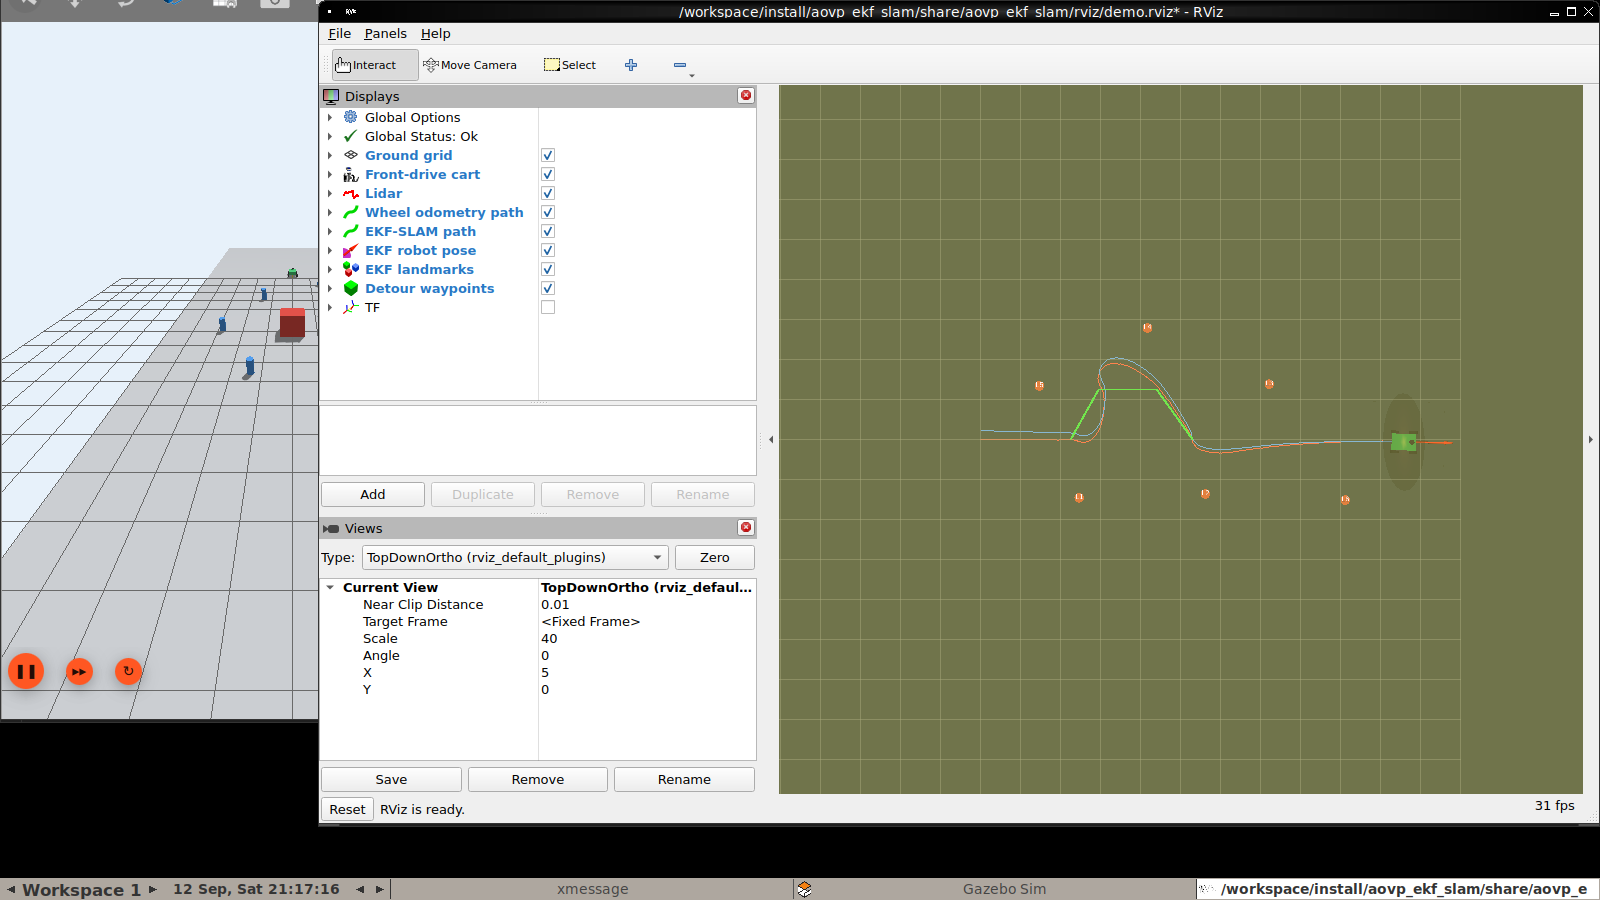
\includegraphics[width=\textwidth]{images/final_run.png}
\caption{Запущенная симуляция Gazebo и визуализация RViz}
\label{fig:rviz}
\end{figure}

\subsection{Траектории}

На рисунке~\ref{fig:trajectory} приведены данные реального прогона. Чёрная линия
соответствует физическому положению модели Gazebo, синяя --- одометрии только по
ведущим колёсам, красная --- оценке EKF-SLAM. На повороте одометрия ведущих
колёс накапливает большую ошибку из-за бокового скольжения. EKF-траектория
остаётся близкой к физической траектории и после манёвра возвращается к $y=0$.

\begin{figure}[H]
\centering
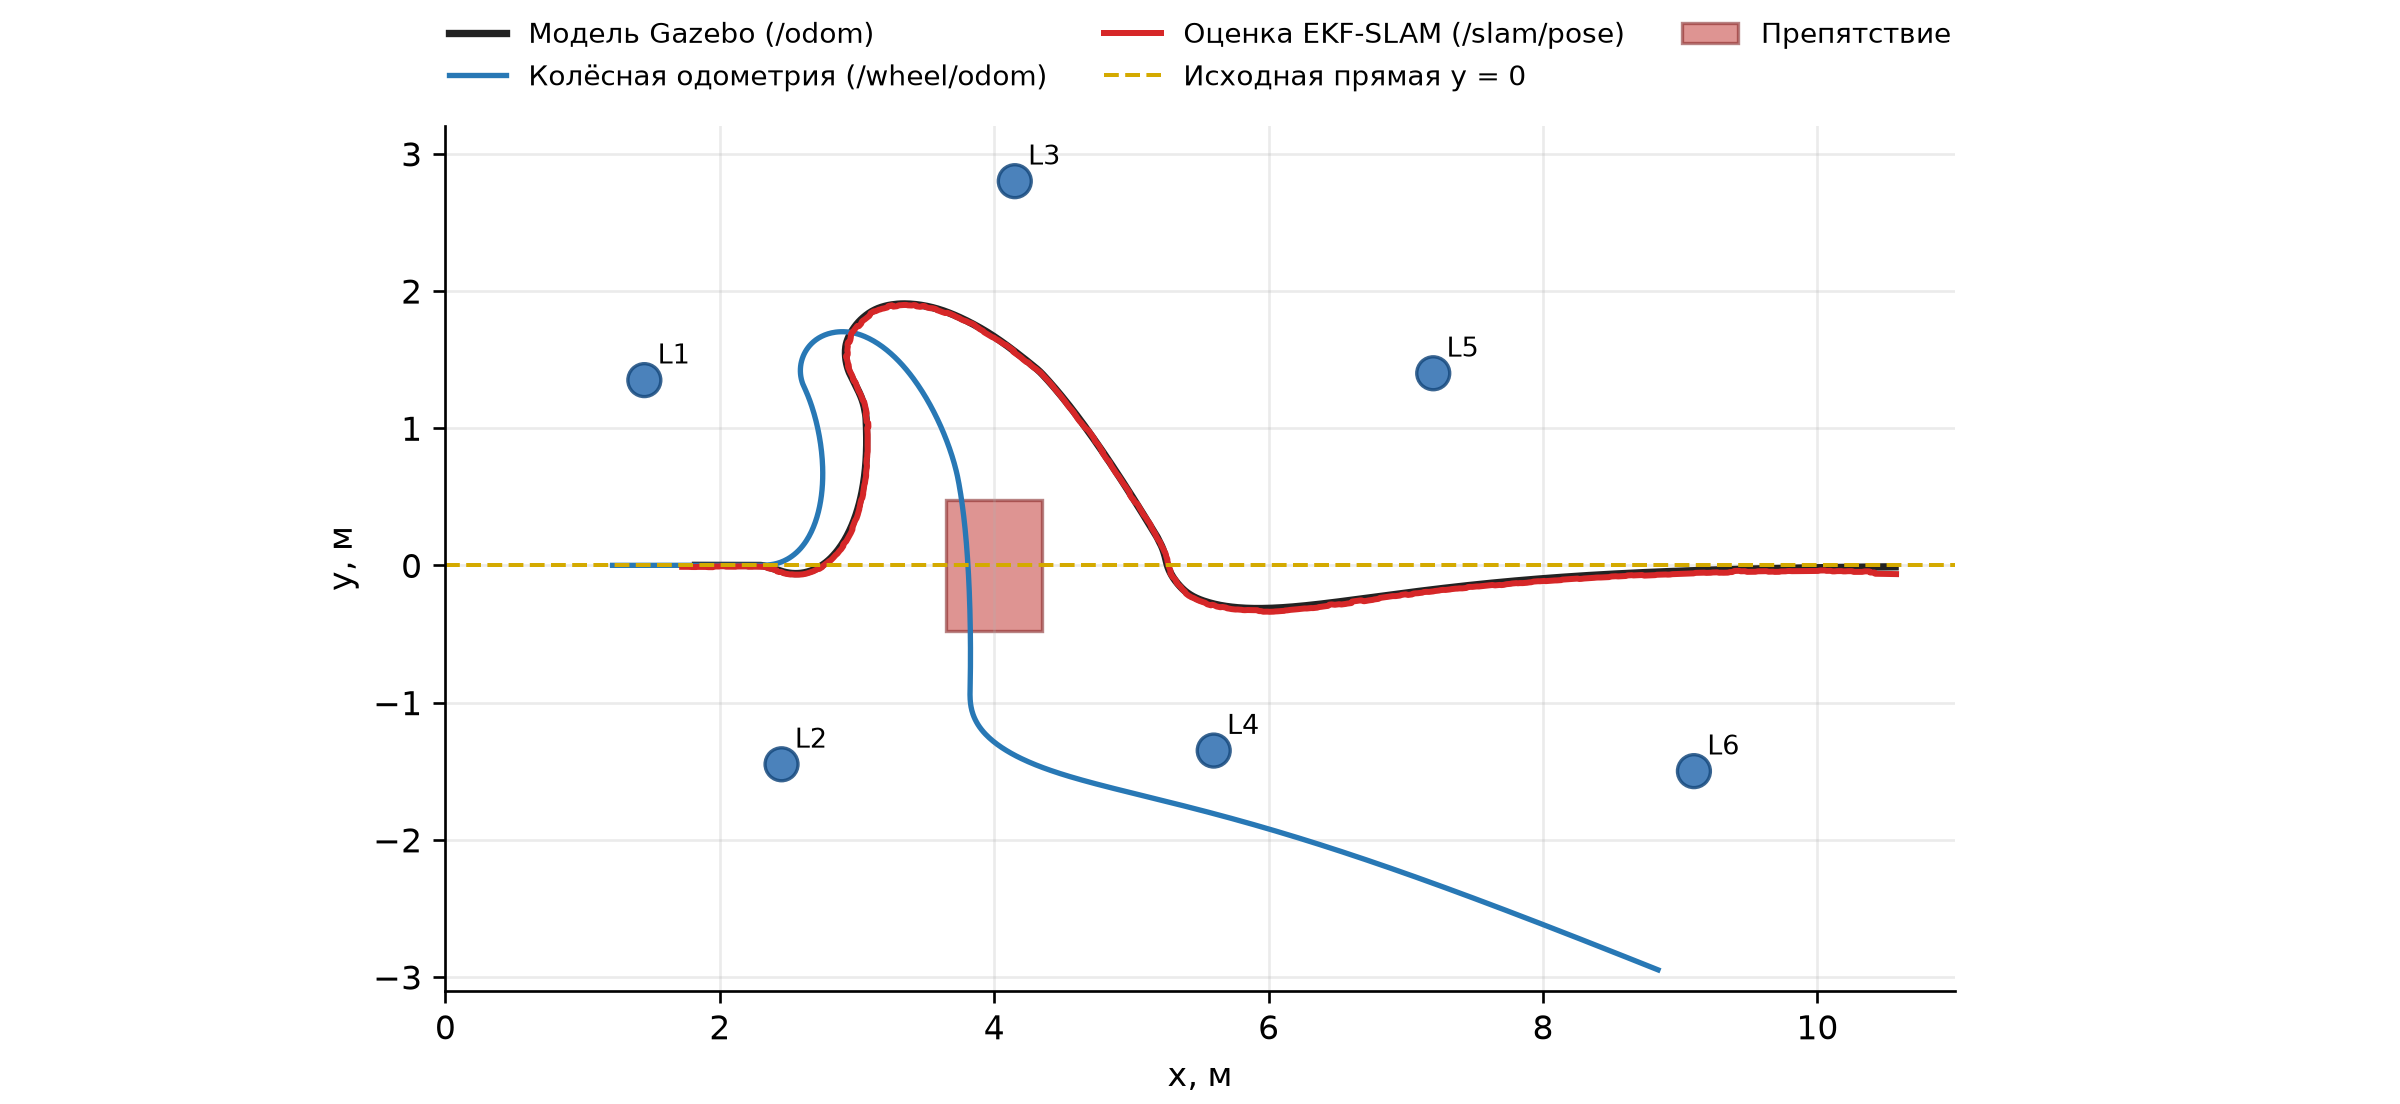
\includegraphics[width=\textwidth]{images/trajectory.png}
\caption{Траектория объезда и оценки положения}
\label{fig:trajectory}
\end{figure}

Максимальное боковое отклонение физической модели составило 1.905~м, поэтому
тележка прошла левее препятствия с достаточным запасом. После объезда она
продолжила движение вдоль исходной прямой и остановилась при $x\approx10.57$~м.

\begin{table}[H]
\centering
\caption{Итоговые координаты экспериментального прогона}
\begin{tabular}{lccc}
\toprule
Источник & $x$, м & $y$, м & Ошибка относительно Gazebo, м \\
\midrule
Gazebo, \texttt{/odom} & 10.566 & -0.011 & 0 \\
Колёсная одометрия, \texttt{/wheel/odom} & 8.838 & -2.948 & 3.408 \\
EKF-SLAM, \texttt{/slam/pose} & 10.573 & -0.064 & 0.054 \\
\bottomrule
\end{tabular}
\end{table}

Финальная позиционная ошибка EKF-SLAM составила 0.054~м, то есть около 0.5\%
пройденного по оси $x$ расстояния. В карту были добавлены все шесть физических
ориентиров.

\subsection{Подтормаживание передних колёс}

Команды колёсам во время того же прогона показаны на
рисунке~\ref{fig:wheels}. В начале объезда скорость левого колеса уменьшается
примерно до 0.4~рад/с, в то время как правое ускоряется до 6.6~рад/с. Затем для
выравнивания курса подтормаживается правое колесо. Ни одно ведущее колесо не
вращается в обратную сторону.

\begin{figure}[H]
\centering
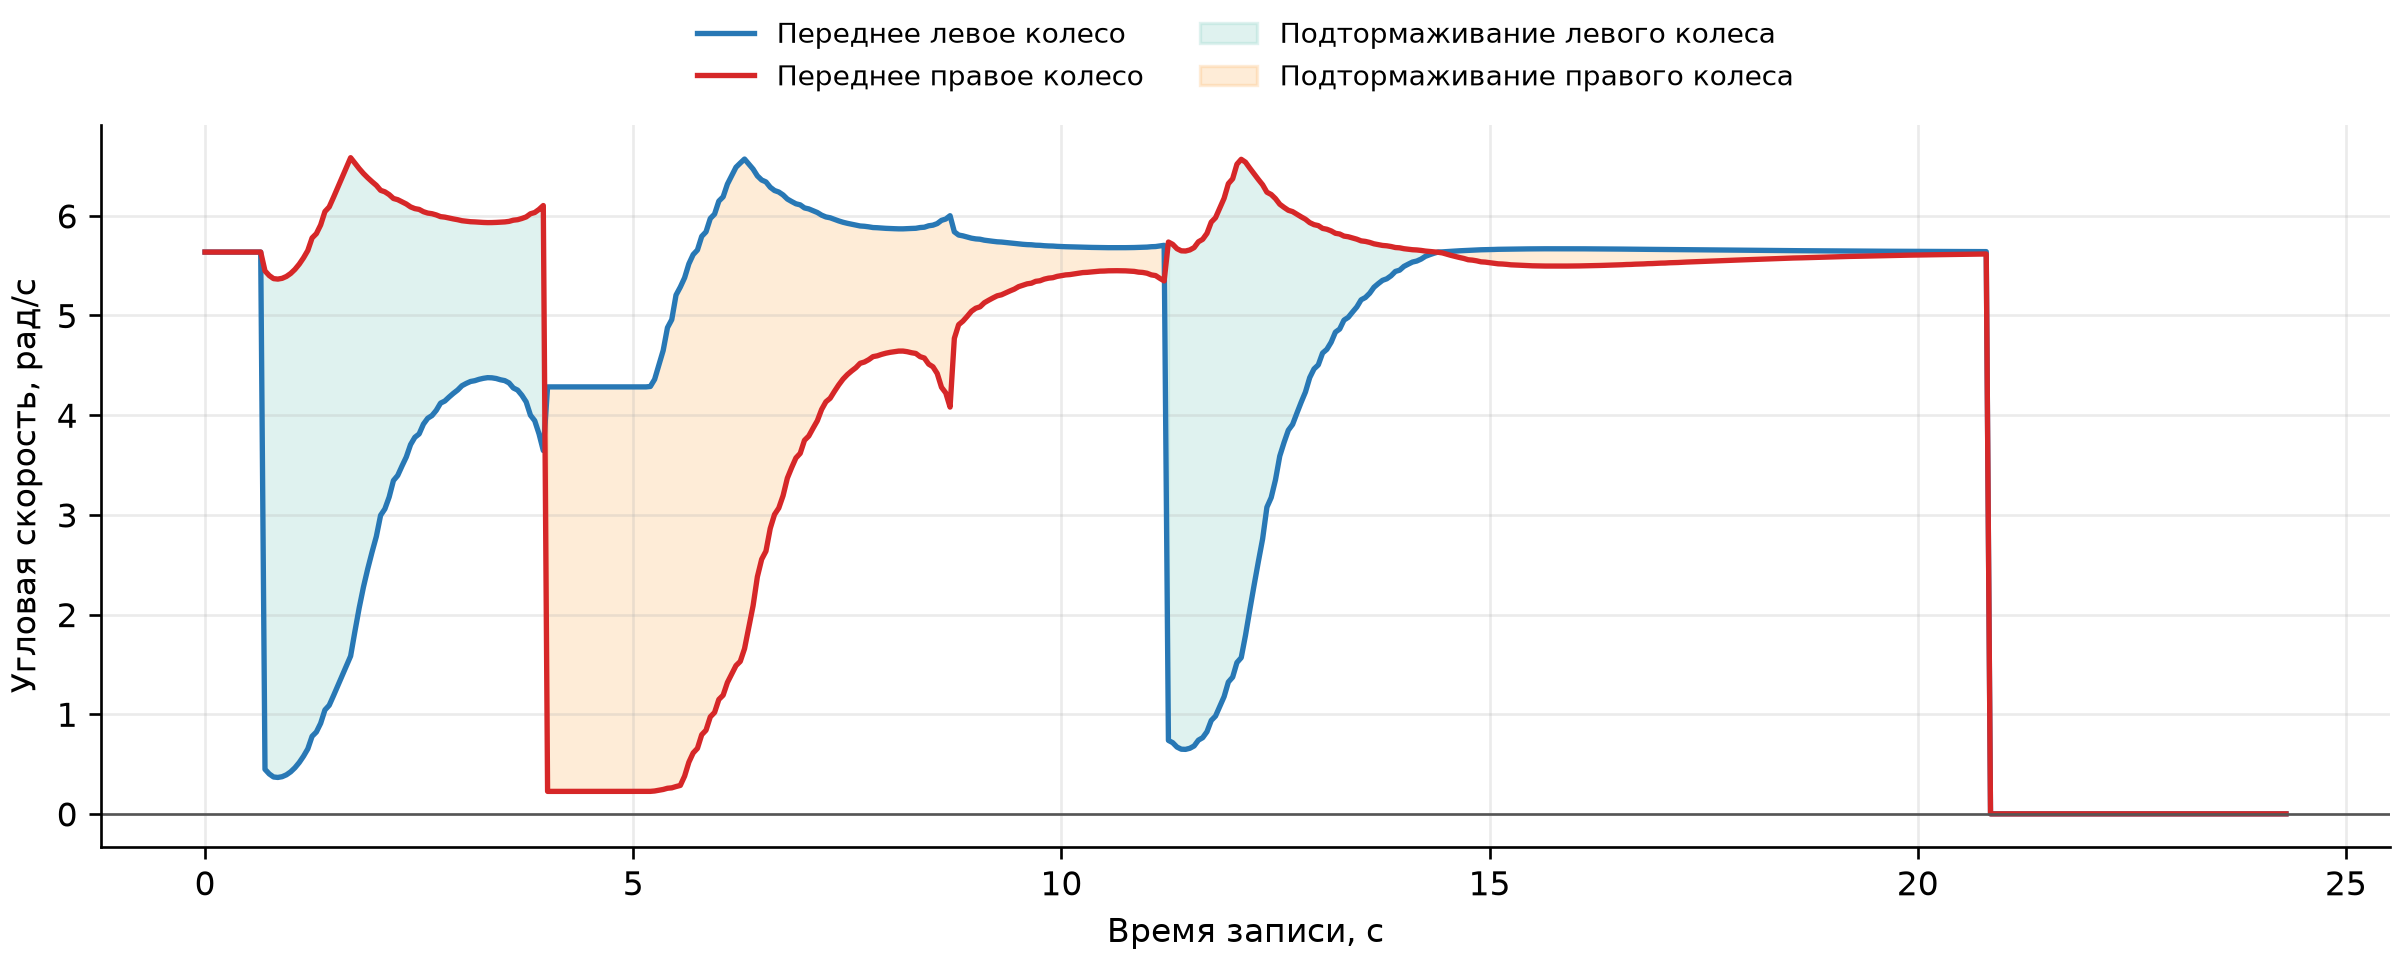
\includegraphics[width=\textwidth]{images/wheel_speeds.png}
\caption{Заданные угловые скорости передних колёс}
\label{fig:wheels}
\end{figure}

\subsection{Автоматические тесты}

Математическая часть EKF и детектор цилиндрических ориентиров отделены от ROS,
что позволяет тестировать их обычным \texttt{unittest}/\texttt{pytest}. В
контейнере выполнена команда

\begin{lstlisting}[language=bash]
colcon test --packages-select aovp_ekf_slam
colcon test-result --verbose
\end{lstlisting}

Пройдено 7 из 7 тестов. Проверяются нормализация углов, prediction, инициализация
ориентира, повторная ассоциация, уменьшение невязки после update, выделение
окружности и отбрасывание невалидных сегментов лидара.

\section{Сборка и запуск}

Для воспроизводимого запуска подготовлены \texttt{Dockerfile} и
\texttt{compose.yaml}. Образ основан на Ubuntu~24.04 и содержит ROS~2 Jazzy,
Gazebo Harmonic, RViz, VNC и noVNC.

Из корневого каталога проекта выполняются команды:

\begin{lstlisting}[language=bash]
docker build -t aovp-ekf-slam:jazzy .
docker run --rm -it --name aovp-ekf-slam \
  --shm-size=1g -p 127.0.0.1:6080:6080 \
  aovp-ekf-slam:jazzy
\end{lstlisting}

После запуска графический рабочий стол доступен по адресу
\url{http://localhost:6080/vnc.html?autoconnect=1\&resize=scale}.

В Ubuntu~24.04 без Docker используются команды:

\begin{lstlisting}[language=bash]
source /opt/ros/jazzy/setup.bash
colcon build --symlink-install
source install/setup.bash
ros2 launch aovp_ekf_slam simulation.launch.py
\end{lstlisting}

Для запуска без графических клиентов можно передать параметры
\texttt{rviz:=false} и \texttt{gz\_gui:=false}.

\section{Заключение}

В работе создана и экспериментально проверена симуляция четырёхколёсной
переднеприводной тележки в ROS~2 и Gazebo. Поворот выполнен без рулевого
механизма и без реверса колёс: курс изменяется за счёт подтормаживания
соответствующего переднего колеса.

Робот автоматически обнаружил препятствие лидаром, прошёл три точки объезда,
вернулся на линию $y=0$ и продолжил прямолинейное движение до $x=10.5$~м.
Классический EKF-SLAM сформировал карту из шести ориентиров и оценил конечную
позицию с ошибкой 0.054~м относительно физической позы Gazebo. Все семь
автоматических тестов завершились успешно.

Полученный проект полностью воспроизводим в Docker и демонстрирует основные
этапы EKF-SLAM: прогноз по одометрии, выделение ориентиров,
ассоциацию измерений по расстоянию Махаланобиса, расширение состояния и
коррекцию по наблюдениям.

\end{document}
